\documentclass[letterpaper]{article}
\usepackage[spanish]{babel}
\selectlanguage{spanish}
\usepackage[utf8]{inputenc}

\usepackage{lipsum}
\usepackage{amsmath,amssymb,amsfonts,amsbsy}
\usepackage{array}
\usepackage{graphicx}
\usepackage{subfigure}
\usepackage{float}
\usepackage{hyperref}

\graphicspath{ {./figures/} }

%\usepackage[pass]{geometry}
\usepackage[left=1.25in,right=1.25in,top=1.0in,bottom=1.0in]{geometry}
\usepackage{listings}

% Custom colors
\usepackage{color}
\definecolor{deepblue}{rgb}{0,0,0.65}
\definecolor{deepred}{rgb}{0.7,0,0}
\definecolor{deepgreen}{rgb}{0,0.6,0}

\newcommand{\mytitle}{Tarea 1}
\newcommand{\myauthor}{Mariana Ortega}
\newcommand{\mydate}{\today}

\begin{document}

\begin{minipage}[t]{.13\textwidth}
	\vspace{-0.25in}
	\begin{figure}[H]
	
\includegraphics[width=0.90\textwidth]{LogoUC.jpg}
	\end{figure}
\end{minipage}
\hfill
\begin{minipage}[t]{.85\textwidth}
    \vspace{0pt}
    \begin{flushleft}
      \begin{tabular}{l}
	{\sc Pontificia Universidad Cat\'olica de Chile}\\
  	{\sc Escuela de Ingenier\'ia}\\
  	{\sc Departamento de Ingenier\'ia Industrial y Sistemas}\\
 	 {\sc ICS1113-Optimizaci\'on}
 \end{tabular}
	\end{flushleft}
\end{minipage}
\vspace{0pt}
\hfill
\vspace*{6cm}
\begin{center}{}
\vspace*{2mm}
{\Huge\bf Informe 4}\\
\vspace*{4mm}
\hrule\vspace*{1pt}\hrule
\vspace*{4mm}
{\LARGE\bf Minimización de los costos para alimentación saludable en colegios financiados por JUNAEB }\\
\vspace*{4mm}
{\huge\bf Grupo 85 }\\
\vspace*{1mm}
\end{center}

\vspace*{30mm}
\begin{flushright} 
	
Guillermo Alfaro Tejerina / 16206843 / sección 2 \\
Gonzalo Balladares Velásquez /	2262595J / sección 1\\ 
Fernanda Galindo Quinteros / 21626448 / sección 1 \\
Nicolás Lavandero Camus	/ 22625879 / seccion 1\\
Guillermo Madariaga Muñoz / 15205304 / sección 5\\

Mauricio Segura Rojas / 2164263J / sección 1\\

 
\vspace*{5mm}
{\large Fecha entrega: 21 de junio de 2024\\}
\end{flushright}

\newpage


\tableofcontents
\newpage
\section{Descripción del problema}
    \subsection{Contexto}
    Las prácticas relacionadas con la alimentación saludable cuando se dan en etapas tempranas en la vida de un individuo establecen los cimientos de la salud y la nutrición idónea para las etapas futuras de su desarrollo. En caso contrario, es decir, descuidar este importante tópico, se puede adquirir resultados adversos expresados en un impacto negativo a largo plazo del impacto en la salud.
\\

Uno de los muchos desafíos que resultan evidenciables en torno a la educación en Chile y que requieren de un análisis exhaustivo es la situación que se presenta en la alimentación escolar. Actualmente, existe un nivel alarmante en cuanto a las tasas de obesidad y desnutrición infantil en Chile, puesto que, según el colegio de nutricionistas, cerca del 58\% de los niños presenta algún problema de malnutrición (Colnut, 2022). Dicho problema radica en un exceso o deficiencia en la alimentación respectivamente, lo cual a su vez se debe a los altos costos en los alimentos más saludables, y el mayor acceso a alimentos ultraprocesados, principalmente compuesto por alimentos altos en calorías, grasas saturadas, azúcares, sodio (sopaipillas, papas fritas, etc.). Según la encuesta Casen del 2022, al año 2020 hubo en aumento de un 2.6\% en la desnutrición en niños (Ministerio de Desarrollo Social y Familia, 2022), siendo más proclive a tener enfermedades de tipo crónico, tales como problemas cardiovasculares, respiratorios, cáncer y diabetes, que en su conjunto representan el 74\% de las causas de muerte a nivel global (WHO, 2023).  
\\

Por otro lado, se destaca la estrecha relación entre la alimentación y el rendimiento físico, y en particular académico. Según datos recientes, en Chile se consume un promedio de 1796 calorías por día, lo cual representa aproximadamente un 92.1\% de la ingesta calórica recomendada para niños en edad escolar (Mayo Clinic, 2022).  
\\

Existen instituciones a cargo de velar por la adecuada alimentación en la etapa escolar (sala cuna y jardín infantil, escolares básica y media). Dado que gran parte de la responsabilidad en cuanto a la alimentación recae en los padres, y que muchas familias se ven afectadas por problemas económicos, es que desde el gobierno existe JUNAEB, un organismo público encargado de ser un soporte estratégico para velar por un correcto proceso educativo para los niños y jóvenes de Chile. A través de sus estudios en el área de alimentación infantil, han llevado a cabo un programa de alimentación escolar importante que día a día abastece a cientos de colegios subvencionados a lo largo del territorio nacional, y que cuenta con un menú completo en cuanto a nivel nutricional para cuidar de la buena alimentación de los estudiantes. Además, cabe destacar que el desayuno de media mañana y el almuerzo proporcionados por la JUNAEB cubren aproximadamente el 50\% de la alimentación diaria recomendada para un niño. Sin embargo, frente al alza de los precios de los alimentos, surge la interrogante de cómo minimizar los costos semanales de alimentación de los estudiantes, asegurando un correcto aporte nutricional. 
    \subsection{Beneficios de resolver el problema}
    Resolver esta interrogante tiene mayor relevancia, ya sea para aumentar o disminuir el dinero invertido en la alimentación de los escolares, pues una correcta alimentación en los estudiantes puede generar una notable mejora en su rendimiento cognitivo (Bryan et al., 2004). Esto debido a que una correcta ingesta de los nutrientes esenciales para el desarrollo, según las pautas indicadas por el ministerio de salud, junto con una racionalización adecuada de las comidas durante el día, permite un correcto funcionamiento del sistema nervioso central, el cual corresponde al mayor determinante en temas de rendimiento académico (García, 2011). Con base en estos datos, se puede concluir que una correcta alimentación de los estudiantes es de suma relevancia para su proceso de aprendizaje. Sin embargo, una correcta alimentación puede ser costosa. A partir de esta premisa se deriva el modelo de optimización expuesto en el presente documento.\\
    
    Dada la creciente preocupación por la salud de los escolares, en relación con las altas tasas de malnutrición, es que la implementación de nuestro modelo de planificación alimentaria saludable, que incluye la entrega de desayunos, almuerzos y colaciones nutritivos, pretende causar un impacto positivo directo a los más de 460 mil alumnos que sufren de sobrepeso y malnutrición (Cigarroa et al., 2017). Pero el alcance global de esta iniciativa busca alcanzar una transformación de los hábitos alimenticios del total de los escolares que estudian en establecimientos donde opera la Junaeb, cifra que equivale a 1.112.783 escolares a nivel nacional (BCN, s.f.). Es por esto que, a partir del análisis de las colaciones de los estudiantes, estas demuestran que poseen un alto contenido de materia grasa, con elevado contenido de grasas saturadas y bajos contenidos de proteínas y fibras dietéticas (Ratner et al., 2013). Por consiguiente, al clasificar los nutrientes de un valor nutricional positivo y negativo en las comidas, estableciendo que estos sean priorizados y eludidos respectivamente, se lograría disminuir los porcentajes de obesidad del grupo objetivo de estudiantes.
    \subsection{Decisiones para lograr el objetivo}
    Para conseguir una reducción en los costos de alimentación saludable a los cuales tendría que incurrir la JUNAEB, se deben tomar decisiones respecto de las proporciones de los distintos tipos de alimentos con los que se estaría alimentando a los estudiantes durante la semana, respetando las cantidades mínimas de aquellos nutrientes que sean positivos, y no exceder las cantidades máximas de nutrientes negativos, velando por una adecuada variedad respecto de los menús que incluirían dichos tipos de comida.  

    \subsection{Enunciado Tipo prueba}
    La JUNAEB es el organismo encargado de la alimentación de los estudiantes de colegios municipales a lo largo de todas las regiones de R. El modelo presentado se encarga de los alimentos que reparte este organismo y los costos de estos a lo largo de un año, donde se consideran los días $D$ de las semanas $M$, definiendo una variable $y_{j,d,m}$ que muestra si hay clases en este día $d$ de la semana $m$. Para el correcto funcionamiento de este modelo se considera que un año tiene 52 semanas, además de que existe un menú diario que cumplir, y que la comida de este se entrega los días antes del día correspondiente. Los alimentos usados tanto en almuerzos como en desayunos se encuentran en el conjunto $J$, donde además estos alimentos deben cumplir ciertos requerimientos nutricionales, basados en los nutrientes del conjunto $F$ , siendo este la cantidad mínima de nutrientes $b_{f}$ y el aporte de cada alimento de estos nutrientes $a_{f,j}$. Además, cada alimento presenta un costo $c_{j,r}$ de compra, un costo $g_j$ de almacenamiento y una disponibilidad $n_{j,m}$ dependiendo del lugar en el que se ubique el colegio y la época del año, por lo que existe una variable $w_{j,d,m}$ que representa la compra del alimento $j$, la cual no puede ser mayor a esta disponibilidad. También se considera que la JUNAEB tiene un presupuesto anual $P$ del que no se puede pasar, por lo que los gastos no deben ser mayores a este, y se considera una demanda $q_{d,m}$ la cual debe ser cubierta por nuestra cantidad de comida enviada $x_{j,d,m}$ en su totalidad si es que se come la comida $j$, por lo que para cumplir esta condición se crea la variable $z_{j,d,m}$ la cual nos indica si se debe enviar este alimento $j$ o no. Finalmente, el modelo considera viable el guardar comida a lo más por una semana en un inventario, definido por la variable de inventario $I_{j,d,m}$ la cual va cambiando de forma diaria cuando se compra y envía comida a los colegios. 

\section{Supuestos}
\vspace{0.3cm}
1.- Se garantiza la llegada de la comida del día durante el transcurso del día anterior, sin ahondar en factores asociados a su transporte.

\vspace{0.3cm}
2.- Cada comida se entrega por día, considerando que esta llegará siempre el día anterior.

\vspace{0.3cm}
3.- La cantidad de niños se mantiene constante en el colegio a lo largo del tiempo, es decir, si algún alumno abandona llegará uno nuevo a reemplazarlo.

\vspace{0.3cm}
4.- Se considera que hay 52 semanas en un año.

\vspace{0.3cm}
5.- La comida almacenada en inventario por más de una semana se desecha.

\vspace{0.3cm}
6.- Se considera un único menú de comida diario para todos los colegios adscritos a beneficio JUNAEB, independiente de la comuna en la que se encuentre.

\vspace{0.3cm}
7.- No existen días feriados.

\section{Modelamiento del problema}
    \subsection{Conjuntos}
    
    \text{$F$ : \{Proteína, carbohidratos, vitaminas, minerales, calcio, magnesio, grasas, sodio, azúcares\}}\\
    

    \begin{minipage}{1.1\linewidth}
    \setlength{\parindent}{0em} 
    $J$ : \{Carne, pavo, chancho, pollo, atún, huevo, porotos, puré, arroz, fideos, papas, lentejas, zanahoria, lechuga, tomate, brócoli, coliflor, apio, manzana, plátano, pera, naranja, durazno, piña, leche, yogurt, flan, arroz con leche, mousse, pan, cereal, galletones, barritas\}     
\end{minipage}
\\

    \text{$D$ : Día = \{1-5\}}\\
    
    \text{$M$ : Semana = \{1-52\}}\\

    \text{$R$ : Región  = \{I - XVI\}}\\
    
    
    \subsection{Parámetros}
    
    \text{$b_{f}$ : Cantidad mínima del nutriente f}\\
    
    \text{$c_{j,r}$ : Costo del alimento j en la región r}\\
    
    \text{$a_{f,j}$ : Aporte del nutriente f del alimento j}\\
    
    \text{$P$ : Presupuesto anual Junaeb: 300.566.878 miles de pesos}\\

    \text{$q_{r,m}$ : Demanda de porciones totales de la región r, en la semana m}\\

    \text{$n_{j,m}$ : Disponibilidad del alimento j durante la semana m}\\
    
    \text{$g_{r,j}$ : Costo de almacenar en la región r el alimento j}\\

    \text{$y_m$ : Indica si hay clases en la semana m}\\
    
    \subsection{Variables}

    $w_{j,d,m}$ : Cantidad de alimento $j$ comprado el dia $d$ en la semana $m$\\
    
    $x_{j,d,m,r}$ : Cantidad del alimento $j$ que se entrega el dia $d$ de la semana $m$ en la region $r$. \\

    
    $I_{j,d,m,r}$ : Cantidad del alimento $j$ que se almacena el dia $d$ en la semana $m$ en la region $r$. \\

    \[
    z_{j,d,m}:
    \begin{cases}
        1 & \text{si se come $j$ el dia $d$ de la semana $m$} \\
        0 & \text{en otro caso}
    \end{cases}
    \]

    
    \subsection{Función objetivo}
    Minimizar los costos semanales de la alimentacion de los estudiantes, manteniendo un correcto aporte nutricional.

    
    \begin{equation*}
    min \sum_{j \in J}\sum_{d \in D}\sum_{m \in M}\sum_{r \in R}{c_{j,r} * x_{j,d,m,r} + g_{r,j} * I_{j,d,m,r} }
    \end{equation*}

    \subsection{Restricciones}
    \begin{enumerate}
    \item La cantidad de nutrientes calificados como positivos deben ser iguales o superiores a la recomendación:
        \begin{equation*}
            \sum_{j \in J} x_{j,d,m,r}* a_{f,j}  \geq b_{f} \qquad \forall d \in D, \forall m \in M, \forall r \in R, \forall f \in F : f < 7
        \end{equation*}
    
    \item Los alimentos no se pueden repetir excesivamente en una semana: 
        \begin{align*}
            z_{j,m,d} \neq z_{j,(d+1),m} \qquad \forall j \in J, \forall d \in D - \{5\}, \forall m \in M
        \end{align*}    
    \item Relación entre variable X y parámetro Y: 
        \begin{align*}
            x_{j,d,m,r} \geq y_m \qquad \forall j \in J, \forall d \in D, \forall m \in M, \forall r \in R
        \end{align*}           
    \item El gasto anual no puede superar el presupuesto dado: 
        \begin{equation*}
            \sum_{j \in J}\sum_{d \in D}\sum_{m \in M}\sum_{r \in R}{C_{j,r} * X_{j,d,m,r} + g_{r,j} * I_{j,d,m,r} } \leq P
        \end{equation*}
    \item Se debe satisfacer la demanda:
        \begin{equation*}
            \sum_{j \in J} (x_{j,d,m,r} + I_{j,d,m,r}) \geq q_{r,m} \qquad  \forall d \in D, \forall m \in M, \forall r \in R  
        \end{equation*}
    \item No se puede comprar mas de la comida disponible:
        \begin{equation*}
            \sum_{d \in D} w_{j,d,m} \leq n_{j,m} \qquad  \forall m \in M, \forall j \in J
        \end{equation*}
    \item El inventario parte vacío:
        \begin{equation*}
            I_{j,1,1,r} = 0 \qquad \forall j \in J, \forall r \in R
        \end{equation*}
    \item La primera semana el inventario funciona de la siguiente manera:
        \begin{equation*}
            I_{j,d,1,r} = I_{j,(d-1),1,r} + w_{j,d,1} - x_{j,d,1,r} \qquad \forall j \in J, \forall r \in R, \forall d \in D -\{1\}
        \end{equation*}
    \item A partir de la semana 2 la comida se guarda en el inventario de la siguiente manera:
        \begin{equation*}
            I_{j,d,m,r} = I_{j,(d-1),m,r} + w_{j,d,m} - x_{j,d,m,r} \qquad \forall j \in J, \forall d \in D -\{1\}, \forall r \in R, \forall m \in M - \{1\} 
        \end{equation*}
    \item Los almuerzos deben ser completos y contener todos los tipos de alimentos disponibles.
        \begin{align*}
            \sum_{j = 1}^{6} z_{j,d,m} = 1 \qquad \forall d \in D, \forall m \in M \\
             \sum_{j = 7}^{12} z_{j,d,m} = 1 \qquad \forall d \in D, \forall m \in M \\
              \sum_{j = 13}^{18} z_{j,d,m} = 1 \qquad \forall d \in D, \forall m \in M \\
              \sum_{j = 19}^{24} z_{j,d,m} = 1 \qquad \forall d \in D, \forall m \in M \\
        \end{align*}
    \item Los desayunos deben ser completos y contener todos los tipos de alimentos disponibles.
        \begin{align*}
            \sum_{j = 25}^{29} z_{j,d,m} = 1 \qquad \forall d \in D, \forall m \in M \\
            \sum_{j = 30}^{33} z_{j,d,m} = 1  \qquad \forall d \in D, \forall m \in M \\
        \end{align*}
    \item Naturaleza de las variables:
        \begin{align*}
            w_{j,d,m} \geq 0 &\qquad \forall j \in J \forall d \in D, \forall m \in M \\
            x_{j,d,m,r} \geq 0 &\qquad \forall j \in J \forall d \in D, \forall m \in M, \forall r \in R  \\
            I_{j,d,m,r} \geq 0 &\qquad \forall j \in J \forall d \in D, \forall m \in M, \forall r \in R  \\
            y_{m} \in \{0,1\} &\qquad \forall m \in M  \\
            z_{j,d,m} \in \{0,1\} &\qquad \forall j \in J, \forall d \in D, \forall m \in M \\
        \end{align*}
\end{enumerate}

    \subsection{Definición de datos}
    Se efectuó un estudio para determinar el requerimiento nutricional diario de proteínas, carbohidratos, vitaminas, minerales, grasas, sodio y azúcar, de infantes de 10 a 13 años (USDA, 2020, pp. 94-96; NIH, 2023). Como nuestro plan de alimentación pretende cubrir un 70\% de la alimentación de los estudiantes, se multiplica por este valor para obtener el archivo de requerimientos nutricionales (archivo requerimientos\_nutricionales).
    \\
    
    A partir de una segunda tabla que señala la cantidad de cada nutriente presente en 100 gramos de cada alimento (USDA, 218). Se puede establecer una relación entre ambas tablas, donde se obtiene una tercera con la cantidad, en gramos, de cada alimento (porción) para alcanzar a cumplir los nutrientes recomendados (archivo aportes\_nutricionales). La siguiente tabla se obtuvo a partir del precio de cada alimento por 100 g del mismo (Odepa, 2024) por cada región (archivo costos).
    \\
    
    A raíz de la búsqueda de la cantidad de alumnos (BCN, s.f.) del ciclo que estamos analizando (5º a 8º básico) por cada región, se multiplicó esta cantidad por las dos comidas diarias entregadas y por 5 días para generar una tabla con la demanda de alimentos semanales ($archivo demanda_comida$).
    Para establecer el valor del almacenamiento, se estimó que se va a requerir una bodega de 200 m2 para alimentos refrigerados y otra idéntica para no refrigerados, con un costo de arriendo  mensual de 0.3 UF/m2 y 0.145 UF/m2 respectivamente (GPS, 2024).  A continuación, se halló una variación entre los precios de arrendamiento de bodegas por región, asignando a la región con un costo menor con un ponderador 1 y al resto de las regiones se les asignó un ponderador superior al 1, de esta manera, obtener el valor mensual del arriendo de ambas bodegas por cada región (archivo costos\_almacenamiento).
    Para elaborar el archivo de disponibilidad, se consideró el total de la producción del alimento destinado al consumo nacional, dividido equitativamente entre todas las regiones y las 52 semanas del año (archivo disponibilidad).

    \subsection{Resultados}
    Al ejecutar el código con los parámetros señalados, obtuvimos una solución factible, que corresponde al valor óptimo 119.138.729.445 pesos chilenos, valor que es inferior al presupuesto actual de la Junaeb, equivalente a 300.566.878.000 pesos chilenos (BCN, s.f.). Por lo que se aprecia una diferencia positiva de 181.428.148.555. Por lo tanto, el trabajo presentado generará un impacto positivo a 262.411 estudiantes del ciclo que es parte del estudio (BCN, s.f.).

    \subsection{Validación del resultado}
    \begin{figure}[H]
    \centering
    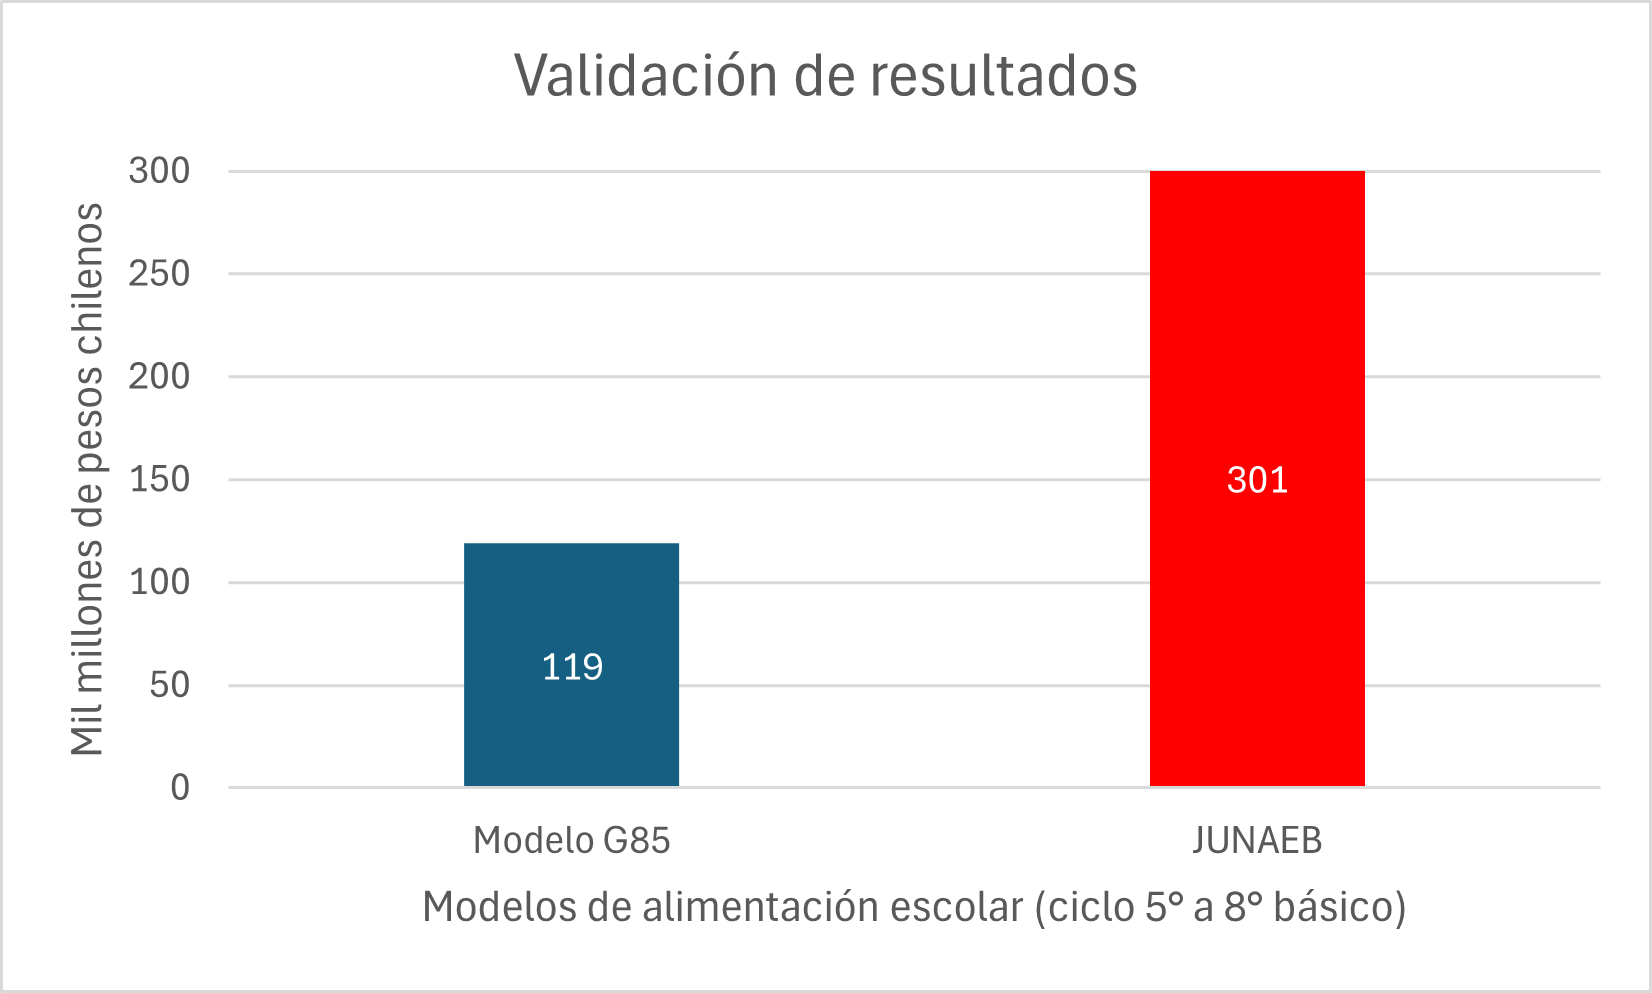
\includegraphics[scale=1]{validacion.png}
    \end{figure}
    En base a los resultados obtenidos al optimizar nuestro modelo en Gurobi, se ha logrado encontrar una solución viable con un valor óptimo de 119.138.729.445 pesos chilenos, lo cual es considerablemente inferior al presupuesto actual de la Junaeb, que asciende a 300.566.878.000 pesos chilenos (BCN, s.f.). Esto resulta en una diferencia positiva de 181.428.148.555 pesos chilenos, generando así un impacto positivo en la alimentación de los alumnos de 5° a 8° básico. La solución obtenida no solo minimiza los costos, sino que también cumple con la problemática planteada, que es asegurar el 70\% de los nutrientes necesarios para un niño de entre 5° y 8° básico.

    Entre los alimentos más consumidos en el programa se encuentran la carne, el pavo, los porotos, las lentejas, la lechuga, el tomate, la piña, la pera, el yogurt y el cereal. La viabilidad y optimalidad de la solución se confirman al cumplir con todas las restricciones impuestas, garantizando que la alimentación proporcionada satisface los requerimientos nutricionales mínimos. Al ser una solución óptima, se asegura que no existe una alternativa que cumpla con las mismas restricciones a un costo menor, demostrando así la eficiencia del trabajo presentado en optimizar los recursos disponibles para el programa de alimentación escolar.

    \subsection{Análisis de Sensibilidad}
    En las tablas a continuación se presenta la configuración original de valor óptimo y alimentos más consumidos, acompañadas de iteraciones en donde se vario algún tipo de parámetro. \\
    Los casos de analisis: costos 2, costos 3, costos 4, costos de almacenamiento 2, costos de almacenamiento 3, disponibilidad 2 y disponibilidad 3, hacen referencia a archivos de excel distnitos que son una variación del archivo original para cada caso y que se adjuntan en la carpeta de la entrega.

    \subsubsection{Variación en los costos de los alimentos}
\begin{table}[H]
\centering
\begin{tabular}{c|c|c|c|}
\cline{2-4}
 & \textbf{Valor Óptimo} & \textbf{Carne} & \textbf{Acompañamiento} \\ \hline
\multicolumn{1}{|c|}{\textbf{Costos Original}} & \$ 119.138.729.445 & Carne & Porotos \\ \hline
\multicolumn{1}{|c|}{\textbf{Costos 2}} & \$ 129.688.372.148 & Pollo & Fideos \\ \hline
\multicolumn{1}{|c|}{\textbf{Costos 3}} & \$ 136.812.079.148 & Atún & Papas \\ \hline
\multicolumn{1}{|c|}{\textbf{Costos 4}} & \$ 190.402.119.604 & Chancho y Pollo & Arroz, Fideos y Lentejas \\ \hline
\end{tabular}
\caption{Variación de costos en los alimentos}
\end{table}

\begin{table}[H]
\centering
\begin{tabular}{c|c|c|c|c|}
\cline{2-5}
 & \textbf{Verdura} & \textbf{Fruta} & \textbf{Lácteo} & \textbf{Desayuno} \\ \hline
\multicolumn{1}{|c|}{\textbf{Costos Original}} & Lechuga y Tomate & Piña & Yogurt & Cereal \\ \hline
\multicolumn{1}{|c|}{\textbf{Costos 2}} & Lechuga & Manzana & Arroz con Leche & Pan \\ \hline
\multicolumn{1}{|c|}{\textbf{Costos 3}} & Lechuga y Apio & Pera & Arroz con Leche & Barritas \\ \hline
\multicolumn{1}{|c|}{\textbf{Costos 4}} & Lechuga, Coliflor y Apio & Manzana y Naranja & Yogurt & Barritas \\ \hline
\end{tabular}
\caption{Continuación de Cuadro 1}
\end{table}

El costo 2 consiste en una variación de costo de los alimentos: huevos, arroz y naranja, que originalmente eran costos mínimos y se convirtieron en costos máximos. Si bien, estos alimentos no estaban dentro de los más consumidos respecto a los costos originales, podemos observar que hubo una nueva planificación y los productos más consumidos tuvieron variación. Además, se observa un leve aumento en el valor óptimo original. \\

El costo 3 consiste en una variación del costo del alimento apio, conservando los cambios hechos en el archivo costos 2. Esta variación, al igual que en el caso anterior, se realizó tomando el alimento con el costo mínimo y convirtiéndolo en el costo máximo. En este caso es interesante observar que, a pesar de cambiar solo el valor de un alimento, el valor óptimo aumenta casi lo mismo que al variar los alimentos anteriores. Además, se puede observar que nuevamente tenemos una configuración nueva de alimentos más consumidos.\\

En el costo 2 y costo 3, se intenta analizar el caso en el cual el alimento más económico se convierte en el más caro, ya que su aumento podría reducir el acceso a ciertos nutrientes, por ende es interesante analizar con qué alimentos se pueden reemplazar y mantener los requerimientos nutricionales.

El costo 4 consiste en una variación por categoría de alimentos, es decir, respecto a los costos originales, se tomó la media de todos los alimentos pertenecientes a la misma categoría, ese valor se le asignó como nuevo precio a los alimentos de la misma categoría, esperando conseguir que la decisión se hiciera por aporte nutricional del alimento dejando de lado el factor relacionado con el precio. Dado el alza de precios de alimentos bajo la media, se puede observar un gran aumento del valor óptimo.\\

\subsubsection{Variación de los costos de almacenamiento}

\begin{table}[H]
\centering
\begin{tabular}{c|c|c|c|}
\cline{2-4}
 & \textbf{Valor Óptimo} & \textbf{Carne} & \textbf{Acompañamiento} \\ \hline
\multicolumn{1}{|c|}{\textbf{Costos Alm. Original}} & \$ 119.138.729.445 & Carne & Porotos \\ \hline
\multicolumn{1}{|c|}{\textbf{Costos Alm. 2}} & \$ 118.964.080.450 & Carne y Chancho & Porotos, Arroz y Lentejas \\ \hline
\multicolumn{1}{|c|}{\textbf{Costos Alm. 3}} & \$ 119.313.378.440 & Carne y Chancho & Porotos, Arroz y Lentejas \\ \hline
\end{tabular}
\caption{Variación de costos de almacenamiento}
\end{table}

\begin{table}[H]
\centering
\begin{tabular}{c|c|c|c|c|}
\cline{2-5}
 & \textbf{Verdura} & \textbf{Fruta} & \textbf{Lácteo} & \textbf{Desayuno} \\ \hline
\multicolumn{1}{|c|}{\textbf{Costos Alm. Original}} & Lechuga y Tomate & Piña & Yogurt & Cereal \\ \hline
\multicolumn{1}{|c|}{\textbf{Costos Alm. 2}} & Zanahoria & Durazno & Yogurt & Cereal y Barritas \\ \hline
\multicolumn{1}{|c|}{\textbf{Costos Alm. 3}} & Zanahoria & Durazno & Yogurt & Cereal y Barritas \\ \hline
\end{tabular}
\caption{Continuación de Cuadro 3}
\end{table}

El costo de almacenamiento 2 consiste en una reducción de los costos de almacenamiento originales en un 20\% para cada región. Mientras que el costo de almacenamiento 3 consiste en un aumento de un 20\% del costo de almacenamiento con respecto al inicial. De esto podemos observar que el valor óptimo presenta leves variaciones, mientras que, por otro lado, podemos ver que los alimentos suelen tener una mayor frecuencia. Con esto se quería analizar el caso en que un costo de un servicio externo variara su valor o fuera susceptible a cambios en el mercado. \\

\subsubsection{Variación en la disponibilidad de alimentos}

\begin{table}[H]
\centering
\begin{tabular}{c|c|c|c|}
\cline{2-4}
 & \textbf{Valor Óptimo} & \textbf{Carne} & \textbf{Acompañamiento} \\ \hline
\multicolumn{1}{|c|}{\textbf{Disponibilidad Original}} & \$ 119.138.729.445 & Carne & Porotos \\ \hline
\multicolumn{1}{|c|}{\textbf{Disponibilidad 2}} & \$ 119.138.729.445 & Carne & Porotos \\ \hline
\multicolumn{1}{|c|}{\textbf{Disponibilidad 3}} & \$ 119.138.729.445 & Carne & Porotos \\ \hline
\end{tabular}
\caption{Variación de disponibilidad}
\end{table}

\begin{table}[H]
\centering
\begin{tabular}{c|c|c|c|c|}
\cline{2-5}
 & \textbf{Verdura} & \textbf{Fruta} & \textbf{Lácteo} & \textbf{Desayuno} \\ \hline
\multicolumn{1}{|c|}{\textbf{Disponibilidad Original}} & Lechuga y Tomate & Piña & Yogurt & Cereal \\ \hline
\multicolumn{1}{|c|}{\textbf{Disponibilidad 2}} & Lechuga y Tomate & Piña & Yogurt & Cereal \\ \hline
\multicolumn{1}{|c|}{\textbf{Disponibilidad 3}} & Lechuga y Tomate & Piña & Yogurt & Cereal \\ \hline
\end{tabular}
\caption{Continuación Cuadro 5}
\end{table}

La disponibilidad 2 consiste en una reducción de un 30\% con respecto a la disponibilidad original. Mientras que la disponibilidad 3 consiste en un aumento de un 30\% con respecto a la disponibilidad original. Se eligió un valor extremo de variación para demostrar que la disponibilidad sigue siendo un valor alto que no representa una limitación al momento de estimar un buen menú. La demanda de alimentos del ciclo escolar analizado siempre se verá cubierta por la alta disponibilidad de alimentos, a pesar de que esta experimente grandes variaciones.
 \\

\section{Conclusión}
Finalmente, este modelo se basa en la selección y distribución de alimentos que cumplan con los requerimientos nutricionales de los estudiantes, mientras se mantiene dentro del presupuesto asignado por la JUNAEB. Es por esto que el modelo es una correcta representación de la realidad, ya que se basa en los parámetros nutricionales mínimos, en los costos de almacenamiento y alimento y por supuesto, en restricciones para validar la variedad de las comidas. \\

Los resultados obtenidos muestra que es factible alimentar a los estudiantes de forma saludable con un costo total de 119.138.729.445, esto es mucho menor al presupuesto anual de 300.566.878.000 pesos. Esto representa una diferencia de 181.428.148.545, lo que propone una optimización efectiva del gasto en alimentación escolar. \\

Por otro lado, se concluye que bajo las condiciones desarrolladas a continuación, la solución es realista e implementable, además de que es robusta frente a cambios en los costos y disponibilidad, ya que se ajusta en base a las restricciones impuestas sin generar grandes diferencias con el valor óptimo original.\\
 
El modelo no solo asegura una nutrición adecuada para los estudiantes, sino que además remarca la importancia de una buena alimentación en el rendimiento académico y la salud a largo plazo de los estudiantes. En esta línea se espera mejorar los hábitos alimenticios de los estudiantes a nivel nacional y reducir las tasas de obesidad y malnutrición.\\ 

Con respecto a las mejoras que se podrían implementar a este proyecto, sería el tema logístico, la capacidad de traslado implementando una red de distribución para aumentar la dificultad. Además de implementar restricciones, como las alergias alimentarias y expandir esto a todos los ciclos escolares. \\

Luego de investigar, se considera que uno de los desafíos para el futuro para un gran sistema, como es la JUNAEB, es implementar un control continuo de las etapas, para que no haya pérdidas de suministros y, por supuesto, implementar las herramientas utilizadas para una mejora continúa. \\

En conclusión, la ejecución de este modelo de planificación alimentaria saludable no es solo financieramente viables, sino que, además, tiene el potencial de causar un impacto positivo muy significativo en la salud y también en el rendimiento académico de los estudiantes en Chile.

\newpage
\section{Bibliografía}

Biblioteca del Congreso Nacional de Chile (BCN). (s.f.). SIIT Estadísticas Territoriales: Matricula según tipo de enseñanza. Recuperado de: https://www.bcn.cl/siit/estadisticasterritoriales//resultados-consulta?id=310555 
\\
\\

Biblioteca del Congreso Nacional de Chile (BCN). (s.f.). Programa Junta Nacional de Auxilio Escolar y Becas. Recuperado de: https://www.bcn.cl/presupuesto/periodo/2024/partida/09/\\capitulo/09/programa/01/montos-reales
\\
\\

Bryan, J., Osendarp, S., Hughes, D., Calvaresi, E., Baghurst, K., y Van Klinken, J. (2004). Nutrients for cognitive development in school-aged children, 295–306. 
\\
\\

Cigarroa, I., Sarqui, C., Palma, D., Figueroa, N., Castillo, M., Zapata-Lamana, R., y Escorihuela, R. (2017). Estado nutricional, condición física, rendimiento escolar, nivel de ansiedad y hábitos de salud en estudiantes de primaria de la provincia del Bio Bío (Chile): Estudio transversal. Revista Chilena de Nutrición. Recuperado de: https://www.scielo.cl/scielo.php?script=sci\_arttext\&pid=S0717-75182017000300209 
\\
\\

Fuente porcentaje obesidad Chile\url{https://elpais.com/chile/2023-06-01/la-obesidad-infantil-un-problema-de-toda-una-sociedad.html\#:\%En\%20esa\%20l\%C3\%B3gica\%2C\%20Chile\%20es,los\%20ni\%C3\%B1os\%20y\%20las\%20ni\%C3\%B1as.}
\\
\\

García, M. (2011). Alimentación y rendimiento escolar en adolescentes. Pasaj Cienc. (14): 99-104.
\\
\\

Global Property Solution (GPS). (2024). Propiedad Código 184.402. Recuperado de: https://gpsproperty.cl/184402
\\
\\

Ibarra, J., Hernández, C. (2019). Hábitos alimentarios y rendimiento académico en escolares adolescentes de Chile. Recuperado de: \url{https://scielo.isciii.es/scielo.php?script=sci\_arttext\&pid=S2174-51452019000400010}   
\\
\\  

Ministerio de Desarrollo Social y Familia. (2022). Población de 0 a 9 años en situación de malnutrición según estado nutricional reportado, según Tramo de edad. \\Recuperado de: https://datasocial.ministeriodesarrollosocial.gob.cl/fichaIndicador/775/1
\\
\\

Mayo Clinic. (2022). Nutrición para niños: pautas para una dieta saludable. Recuperado de: https://www.mayoclinic.org/es/healthy-lifestyle/childrens-health/in-depth/nutrition-for-kids/art-20049335 
\\
\\

National Institutes of Health (NIH). (2023). Dietary Supplement Facts Sheets - Strengthening Knowledge and Understanding of Dietary Supplements. Recuperado de: https://ods.od.nih.gov/factsheets/list-all/
\\
\\

Oficina de Estudios y Políticas Agrarias (Odepa). (2024). Precios - Mejores alimentos de temporada. Recuperado de: https://www.odepa.gob.cl/precios/mejores-alimentos-de-temporada#Arica
\\
\\

Ratner, R., Durán, S., Garrido, M., Balmaceda, S., y Atalah, E. (2013). Impacto de una intervención en alimentación y nutrición en escolares. Revista chilena de pediatría, 84(6), 634-640. Recuperado de: https://www.scielo.cl/scielo.php?script=sci\&pid=S0370-41062013000600006 
\\
\\

U.S. Department of Agriculture (USDA). (2018). Food Data Central Search Results. Recuperado de: https://fdc.nal.usda.gov/fdc-app.html#/food-details/174036/nutrients
\\
\\

U.S. Department of Agriculture y U.S. Department of Health and Human Services (USDA y HHS). (2020). Dietary Guidelines for Americans, 2020-2025 (9th ed.) (pp. 94-96).  Recuperado de: https://www.dietaryguidelines.gov/sites/default/files/2021-03/Dietary_Guidelines_for_Americans-2020-2025.pdf
\\
\\

World Health Organization (WHO). (2023). Noncommunicable diseases. Recuperado de:\\ https://www.who.int/news-room/fact-sheets/detail/noncommunicable-diseases


    

\end{document}
